\section{Background: The EBA Framework}
\label{background-section}
The EBA framework reference provides \textit{shape-and-effect inference} and allows extracting an \textit{effect-annotated control flow graph} (effect-CFG) from a Linux kernel program. The annotated control flow graph can be statically analyzed in order to find possible bugs in the given program. A control-flow-graph is a representation of all paths that might be traversed through a program when executed \cite{cfg}. A node in the graph represents a program point where edges represent a jump in the control flow. 

\newpar Figure \ref{initial-bug-visualisation} shows an example of a bug found in the Linux kernel\footnote{This bug was patched in commit \href{https://github.com/torvalds/linux/commit/4dd75b33}{\texttt{4dd75b33}}.} and the data types provided by the framework. These data types have been used in this thesis to develop new resource manipulation bug checkers. This section will explain the definitions by Abal et. al. \cite{Abal2017EffectiveBF} which I build upon in this thesis in order to develop new bug checkers. 

\begin{figure}[H]
\centering
\begin{minipage}{0.4\textwidth}
    \begin{minted}[fontsize=\scriptsize, breaklines, linenos]{c}
static void orphan_delete(struct ubifs_info *c, struct ubifs_orphan *orph)
{
	if (orph->del) {
		spin_unlock(&c->orphan_lock);
		return;
	}
	if (orph->cmt) {
		spin_unlock(&c->orphan_lock);
		return;
	}
}

void ubifs_delete_orphan(struct ubifs_info *c, ino_t inum)
{
	orphan_delete(c, orph);
	spin_unlock(&c->orphan_lock);
}
\end{minted}
\end{minipage}
\hspace*{0.05\textwidth}
\begin{minipage}{0.45\textwidth}
    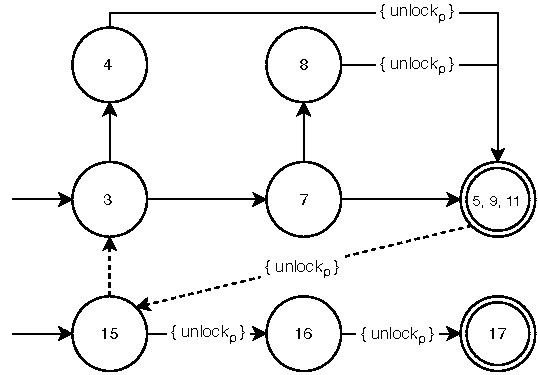
\includegraphics[width=\textwidth]{background/figures/annotated-cfg}
\end{minipage}
\caption{An illustration of a double-unlock bug (\texttt{4dd75b33}) found in the Linux kernel and the analysis data types provided by EBA. The relevant code is shown on the left-hand side and on the right-hand side is the \textit{effect-CFG} with \textit{lock} and \textit{unlock effects} provided by EBA. The numbered CFG nodes show the corresponding line numbers.}
\label{initial-bug-visualisation}
\end{figure}

\newpar I build upon EBA in this thesis. Though it is generally seen as a black box. A certain understanding of definitions described by Abal et. al. \cite{Abal2017EffectiveBF} is required to see how we build upon the existing work. Three main definitions are of note here, namely \textit{shapes}, \textit{regions} and \textit{effects}. EBA employs CIL \cite{cil}, a lightweight intermediate representation of the C code implemented in OCaml. Abal et. al define a base type system for a smaller language than CIL. This chapter will provide a summary of the definitions we also use in this thesis to define our work. 

\newpar The base type language of the \textit{Shape-and-Effect System} is defined to be:  

\begin{equation*}
\begin{aligned}
    \text {l-value types } T^{L} \quad &: \quad \text{ ref } T^{R} \quad | \quad \text{ ref } \left(T_{1}^{R} \times \cdots \times T_{n}^{R} \rightarrow T_{0}^{R}\right)\\
    \text {r-value types } T^{R} \quad &: \quad \texttt{int} \quad | \quad \text{ ptr } T^{L}
\end{aligned}
\end{equation*}

\newpar The l-value ($T^{L}$) types and r-value ($T^{R}$) types correspond to the left and right side of assignments in C. A reference type, $\texttt{ref} \; T$ represents a memory cell, holding objects of the type $T$. For example, $\text{ptr}\;\text{ref}\;T$ is the current address of the reference for the objects T in memory. The corresponding tiny programming language is described by the following grammar:

\begin{equation*}
\begin{aligned}
    \text {l-value expressions } L \quad &: \quad x \quad | \quad f \quad | \quad *E \\
    \text{r-value expressions } E \quad &: \quad n \quad | \quad E_{1}+E_{2} \quad | \quad \texttt{if (}E_0\texttt{)} \; E_1 \; \texttt{else} \; E_2 \quad | \quad (T) E \\
    &| \quad \texttt{new} \: x : T=E_1 ;\: E_2 \quad | \quad !L \quad | \quad \& L \quad | \quad L_1 := E_2 ;\: E_3 \\
    &| \quad \texttt{fun} \:T\:f\:(T_1\:x_1, \cdots, T_n\:x_n) = E_1 ;\: E_2 \quad | \quad L_0(E_1, \cdots, E_n)
\end{aligned}
\end{equation*}

\newpar L-value expressions (L) represent memory locations and will always be assigned reference types ($T^L$). Function values are immutable, while other variables ($x$) are not. $*E$ represents the dereferencing of a pointer, which is looking up the reference cell in memory, as seen in C. R-value expressions are \textit{values}, such as integers ($n$) and pointers. $(T)E$ is a cast, as found in C, and will convert the value $E$ to the type $T$.$new\: x : T = E_1; E_2$ represents the introduction of a new variable, $x$, which is initialized in $E_1$ and available in $E_2$. $x$ is the name of the memory cell where the value of $E_1$ is stored, and has the type $\texttt{ref} \:T$. The expression $!L$ will read an l-value, and pointer values can be obtained with $\&L$.
The assignment expression $L_1 := E_2 ;\: E_3$ allows assigning a new value $E_2$ to the value $L_1$ before evaluating $E_3$. The declaration of a function, $f$, $\texttt{fun} \:T\:f\:(T_1\:x_1, \cdots, T_n\:x_n) = E_1 ;\: E_2$, $f$ will then be visible in $E_2$, similar to \texttt{new}. The function $f$ will bind the parameters $x_1, \cdots, x_n$ and evaluate the body expression $E_1$. Loops and \texttt{goto}s are not modelled in this system. 

\subsection{Regions}
Regions are an abstract representation of memory. Variables are names for memory cells on the stack. Aliasing --- when multiple variable names actually point to the same memory --- can therefore happen. These possibly aliased memory cells are tracked by the shape-and-effect system using regions. The system will assign a region, $\rho$, to each reference value in the source code, and attempt to detect aliased variables, by unioning these regions when it can no longer distinguish the regions.

\subsection{Effects}
Effects represent how expressions affect regions. For example, an expression which reads a memory location will have the effect of reading that region. Likewise, expressions writing to memory locations will have the effect of writing to that region. An example of a set of effects is $\varphi = \{read_\rho , read_{\rho'} , write_{\rho'}\}$, where the region $\rho$ is being read and the region $\rho'$ is being both read and written.

\subsection{Shapes}
\begin{figure}[H]
    \centering
    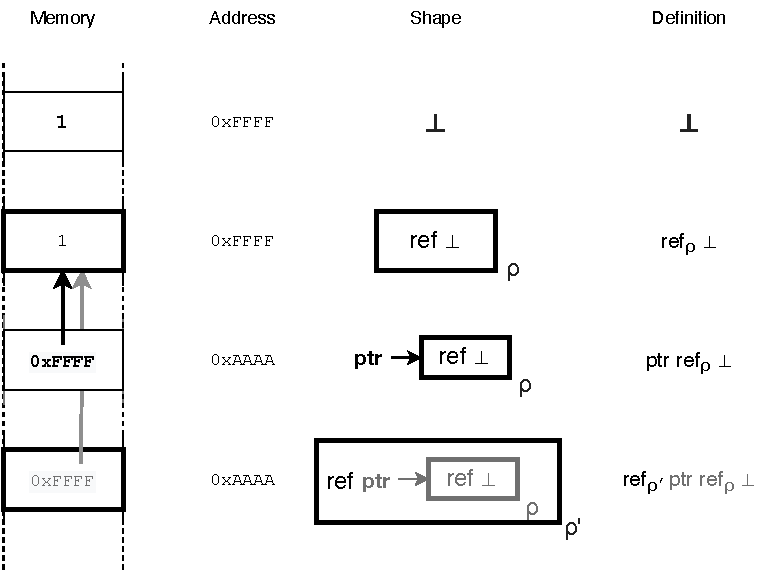
\includegraphics[width=0.7\textwidth]{background/figures/shapes}
    \caption{An illustration of \textit{shapes} and how they represent values in memory. Arrows represent pointers, and bold cells refer to the cell itself, not its contents.}
    \label{shapes-figure}
\end{figure}

\newpar A shape approximates the memory representation of an object, and this shape is fixed and kept across type casts. Shapes are annotated with regions showing a \texttt{"points-to"} relationship between references. Abal et. al. define shapes in the following terms. 

\begin{equation*}
\begin{aligned}
    \text { l-value shapes } Z^L \quad &: \quad \text{ref}_{\rho} \:Z^R \quad | \quad \text{ref}_{\rho}\:(Z_1^L \times \cdots \times Z_n^L \stackrel{\varphi}{\rightarrow} Z_0^R)\\
    \text {r-value shapes } Z^R \quad &: \quad \perp \quad | \quad \text { ptr } Z^L \quad | \quad \zeta
\end{aligned}
\end{equation*} 

\noindent Shapes are also divided into l-value and r-value shapes in a similar fashion as the aforementioned type system, albeit without an integer type and with shape variables, $\zeta$. An r-value is the shape objects where the \textit{atomic} shape, $\perp$, indicates that an object has no relevant structure --- e.g. an integer. A pointer expression has the pointer shape, $\text{ ptr } Z^L$, where $Z^L$ is the shape of the target reference cell of the pointer. This means that a pointer represents the address of a reference cell, and therefore a pointer shape necessarily encloses a reference shape. If a pointer is being cast, its integer value will then have a pointer shape, $\text{ ptr } Z^L$. $\zeta$ represents arbitrary r-value shapes. These definitions and how they represent values in memory are illustrated in Figure \ref{shapes-figure}.

\newpar Functions receive \textit{function shapes},

\begin{equation*}
    \operatorname{ref}_{\rho_{0}}\left(Z_{1}^{L} \times \cdots \times Z_{n}^{L} \stackrel{\varphi}{\rightarrow} Z_{0}^{R}\right),
\end{equation*} 

\noindent where the memory region $\rho_0$ identifies the function and is used by EBA to keep track of calls to the function. Functions need to be allocated a region, due to the use of function pointers in C. 

\newpar Function shapes represent an abstraction of the shapes given to a function as well as the shape of the result of the function. The parameters $Z_{1}^{L} \times \cdots \times Z_{n}^{L}$ correspond to the shapes of parameters the function is given and $Z_{0}^{R}$ is the shape of the result of the function. Since function parameters are stored in stack variables, these parameters are l-value shapes. The \textit{latent effect}, demonstrated as $\stackrel{\varphi}{\rightarrow}$ above represents the effects that may happen when executing the function. Function shape schemes along with the correlation between types and shapes are described in more detail by Abal et. al. \cite{Abal2017EffectiveBF}. 

\newpar An environment $\Gamma$ maps variables $v$ to their corresponding reference shapes: $\Gamma(v) = ref_\rho Z$. $v$ is effect variables, described in the following. As already mentioned, function shapes are represent effects that may happen when executing a function, but this \textit{may} can be made more concrete using function inlining, in which case the actual effects of calling a function within another function can be inferred concretely. The use of inlining is detailed in Section \ref{implementation}. 

\subsection{Shape-and-effect Inference}
Abal et. al. present inference rules $\vdash \subseteq \text { ENV } \times \text { VALUE } \times \text { SHAPE } \times \text { EFFECT }$ for \textit{shape-and-effect inference} \cite{Abal2017EffectiveBF}, which allows determining the shape of a given expression as well as determining what the effects of evaluation the expression are. This is expressed as the judgment 

\begin{equation*}
    \Gamma \vdash E: Z \& \varphi
\end{equation*}

\noindent specifying that under the enviroment $\Gamma$, the value $E$ has the shape $Z$ resulting in the effects $\varphi$.

\newpar In other words, the environment $\Gamma$ keeps track of the values and which effects accompany them. The inference rules defined by Abal et. al., lead to these values having effects accompanying them based on the determining of their shapes. I present two of these inference rules, $\text{[FETCH]}$ and $\text{[ASSIGN]}$, in the following to give an intuition of how the inference system works and how effects are produced. The previously shown examples of effects, $read$ and $write$, are found by the use of these two inference rules, since $\text{[FETCH]}$ and $\text{[ASSIGN]}$ produce the effects of reading from or writing to a given memory region, $\rho$. 

\begin{equation*}
    [\text{FETCH}] \quad \frac{\Gamma \vdash L: \text{ref}_{\rho} Z \& \varphi}{\Gamma \vdash {!L}: Z \& \varphi \cup\left\{r e a d_{\rho}\right\}}
\end{equation*}

\newpar The $\text{[FETCH]}$ rule allows, given a reference to a shape $\text{ref}_{\rho} Z$ in the environment $\Gamma$, that the shape can be dereferenced by the use of the bang-operator $!$, resulting in the shape $Z$. This has the effect of reading the memory region $\rho$, in turn adding a $read_\rho$ effect to the preexisting effects, $\varphi$. Intuitively preserving the preexisting effects makes sense, since the act of reading a value should only produce effects, not remove preexisting effects of determining that value. Computing the value of the form $\text{ref}_{\rho} Z$ could have produced other effects by the use of the other inference rules of the system and these effects therefore need to be preserved.  

\begin{equation*}
    [\text{ASSIGN}] \quad \frac{\Gamma \vdash L: \mathrm{ref}_{\rho} Z \& \varphi_{1} \quad \Gamma \vdash E_{1}: Z \& \varphi_{2} \quad \Gamma \vdash E_{2}: Z' \& \varphi_{3}}{\Gamma \vdash L:=E_{1} ; E_{2}: Z^{\prime} \& \varphi_{1} \cup \varphi_{2} \cup\left\{w r i t e_{\rho}\right\} \cup \varphi_{3}}
\end{equation*}

\newpar $\text{[ASSIGN]}$ allows assigning a value $E_1$ to the value $L$. This will evaluate both expressions $E_1$ and $E_2$, resulting in effects for both $E_1$ and $E_2$ being determined. The result of the assignment is a $\text{write}_\rho$ effect, which is added to the sets of effects of $E_1$ and $E_2$ as well as existing effects of $L$. The left and right-hand sides of the expression, $L$ and $E_1$ must be of the same shape, $Z$, while the result of evaluating $E_2$ can be of a different shape, $Z'$. While the asasignment of a new value to $L$ will bind the value in the environment, the effects of getting to this stage of the inference are still interesting. Assignment leading to producing an effect and not removing preexisting effects makes sense, since effects are produced by computing the value being written, as well as determining what is being written to. $\text{[ASSIGN]}$ will, by the evaluation of $\Gamma \vdash L: \text{ref}_{\rho} Z$, result in both $read$ and $write$ effects being added to the effects $\varphi$, since the value of $L$ is dereferenced by assignment. 

\newpar Abal et. al. axiomize the behaviour of certain operations, $f$, with a signature, $Z_{i}^{L} \stackrel{\varphi}{\rightarrow} Z_0$. The axiom specifies shapes of the input arguments expected by the function, $Z_{i}^{L}$, the shape of the output, $Z_0$, and the resulting effects, $\varphi$. The authors present an example of two axioms for locking and unlocking functions found within the Linux kernel. These axioms are used extensively by the inference system, in order to infer how resource manipulation is used in the kernel. 

\begin{equation*}
\begin{aligned}
        \texttt{spin\_lock}: \quad & \text{ref}_{\rho_1} \text{ptr } \text{ref}_{\rho_2} \zeta \xrightarrow{{\texttt{lock}}_{\rho_2}}\perp \\
        \texttt{spin\_unlock}: \quad & \text{ref}_{\rho_1} \text{ptr } \text{ref}_{\rho_2} \zeta \xrightarrow{{\texttt{unlock}}_{\rho_2}}\perp
\end{aligned}
\end{equation*}

\newpar Axioms have been defined by Abal et. al. for multiple functions in the kernel, allowing inferring what the effects are of using these built-ins. These specify that \texttt{spin\_lock} and \texttt{spin\_unlock} receive pointers as arguments, $\rho_1$, pointing to an object, $\rho_2$. The effects above the arrows indicate that the functions \texttt{lock} and \texttt{unlock} the object in $\rho_2$, respectively.

\newpar Shapes and effects are computed efficiently by EBA using type inference. The shape-and-effect system --- and by extension this thesis --- is implemented for C and not for the tiny language used for the introduction of the definitions above.

\subsection{Effect-CFG Abstraction}
Abal et. al present the \textit{Effect-based Control-Flow Graph ($\varphi$-CFG)}. This is described as a CFG where nodes represent program points and edges specify the control flow, annotated with variables and their memory shapes, and nodes annotated with the effects inferred for their corresponding points.  